\documentclass[10pt]{article}
\usepackage{tikz}
\usetikzlibrary{shapes.misc}
\usepackage[margin=0cm]{geometry}
\pagestyle{empty}
\tikzstyle{every node}=[cross out, draw, red]

\begin{document}

\vspace*{\fill}
\begin{center}
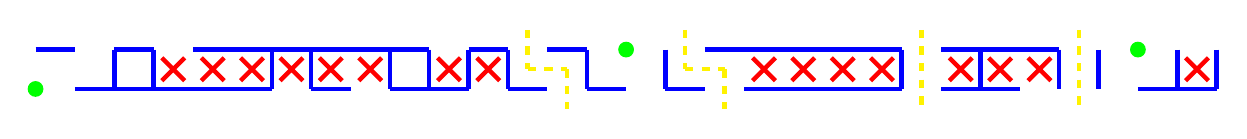
\begin{tikzpicture}[x=0.5cm, y=-0.5cm, ultra thick, blue]
% Walls
    \draw (0,0) -- (1,0);
    \draw (2,0) -- (3,0);
    \draw (4,0) -- (10,0);
    \draw (11,0) -- (12,0);
    \draw (13,0) -- (14,0);
    \draw (17,0) -- (22,0);
    \draw (23,0) -- (26,0);
    \draw (1,1) -- (6,1);
    \draw (7,1) -- (8,1);
    \draw (9,1) -- (11,1);
    \draw (12,1) -- (13,1);
    \draw (14,1) -- (15,1);
    \draw (16,1) -- (17,1);
    \draw (18,1) -- (22,1);
    \draw (23,1) -- (25,1);
    \draw (28,1) -- (30,1);
    \draw (2,0) -- (2,1);
    \draw (3,0) -- (3,1);
    \draw (6,0) -- (6,1);
    \draw (7,0) -- (7,1);
    \draw (9,0) -- (9,1);
    \draw (10,0) -- (10,1);
    \draw (11,0) -- (11,1);
    \draw (12,0) -- (12,1);
    \draw (14,0) -- (14,1);
    \draw (16,0) -- (16,1);
    \draw (22,0) -- (22,1);
    \draw (24,0) -- (24,1);
    \draw (26,0) -- (26,1);
    \draw (27,0) -- (27,1);
    \draw (29,0) -- (29,1);
    \draw (30,0) -- (30,1);
% Pillars
    \fill[green] (15,0) circle(0.2);
    \fill[green] (28,0) circle(0.2);
    \fill[green] (0,1) circle(0.2);
% Inner points in accessible cul-de-sacs
    \node at (3.5,0.5) {};
    \node at (4.5,0.5) {};
    \node at (5.5,0.5) {};
    \node at (6.5,0.5) {};
    \node at (7.5,0.5) {};
    \node at (8.5,0.5) {};
    \node at (10.5,0.5) {};
    \node at (11.5,0.5) {};
    \node at (18.5,0.5) {};
    \node at (19.5,0.5) {};
    \node at (20.5,0.5) {};
    \node at (21.5,0.5) {};
    \node at (23.5,0.5) {};
    \node at (24.5,0.5) {};
    \node at (25.5,0.5) {};
    \node at (29.5,0.5) {};
% Entry-exit paths without intersections
    \draw[dashed, yellow] (12.5,0.5) -- (13.5,0.5);
    \draw[dashed, yellow] (16.5,0.5) -- (17.5,0.5);
    \draw[dashed, yellow] (12.5,-0.5) -- (12.5,0.5);
    \draw[dashed, yellow] (13.5,0.5) -- (13.5,1.5);
    \draw[dashed, yellow] (16.5,-0.5) -- (16.5,0.5);
    \draw[dashed, yellow] (17.5,0.5) -- (17.5,1.5);
    \draw[dashed, yellow] (22.5,-0.5) -- (22.5,1.5);
    \draw[dashed, yellow] (26.5,-0.5) -- (26.5,1.5);
\end{tikzpicture}
\end{center}
\vspace*{\fill}

\end{document}
